% !TEX encoding = UTF-8 Unicode

\documentclass[10pt,a4j]{ltjsarticle}
\usepackage{url}
\usepackage{graphicx}
\usepackage{float}
\usepackage{listings}

\renewcommand{\figurename}{図}
\renewcommand{\tablename}{表}
\renewcommand{\lstlistingname}{プログラム}

% the header name for the list of it.
\renewcommand{\listfigurename}{図目次}
\renewcommand{\listtablename}{表目次}
\renewcommand{\lstlistlistingname}{プログラム目次}

\begin{document}
\lstset{
  basicstyle = \ttfamily,
  numbers = left,
  frame = single
}
%表紙
\begin{titlepage}
  \begin{center}  
    \vspace*{20truept}    
    {\LARGE 2022年度 卒業論文}
    
    \vspace*{75truept}    
    {\Huge Scratchからの移行を意識した} %論文タイトル
    
    \vspace{10truept}
    {\Huge プログラミング言語の開発} %論文タイトル 長い場合 改行1
    
    \vspace{10truept}
    {\Huge } %論文タイトル 改行2
    
    \vspace{85truept}
    {\LARGE 指導教員 須田 宇宙 准教授} 
    
    \vspace{60truept}
    {\LARGE 千葉工業大学 情報ネットワーク学科}
    
    \vspace{15truept}
    {\LARGE 須田研究室}
    
    \vspace{70truept}
    {\LARGE 1932034 氏名 川原 史哉 } % 氏名は消さない 学生番号 氏名 
    
    \vspace{70truept}
  \end{center}
  \begin{flushright}
    {\LARGE 提出日 2023年1月17日}
  \end{flushright}
\end{titlepage}

%目次
\setcounter{tocdepth}{3} %目次の深さ設定
\thispagestyle{empty} %ページスタイルの変更
\tableofcontents %目次の作成
\thispagestyle{empty} %ページスタイルの変更
\listoffigures
\thispagestyle{empty} %ページスタイルの変更
\listoftables
\thispagestyle{empty} %ページスタイルの変更
\lstlistoflistings
\clearpage %改ページ

\setcounter{page}{1} %ページ番号を0から始める
\section{緒言}
%背景
近年の急速な情報化に伴い,2020年度から小学校ではプログラミング教育の必修化が行われた.これにより小学生でも扱いやすいビジュアルプログラミング言語が注目されている.
代表的なビジュアルプログラミング言語に「Scratch」がある.「Scratch」は指示の書かれたブロックを並べることで視覚的にわかりやすく,直感的な操作でプログラミングができる.また,文字のタイピング量が少ない点や英単語の知識を必要としない点などから,初学者のプログラミング学習に適している.

%問題点
本格的なプログラムを作成していくうえで,テキストプログラミング言語の学習が必要になる.しかし,Scratchに慣れていると,テキストプログラミング言語の学習を始めようとしたときに仕様の違いが挫折の要因になり得ると考えた.例えば,スプライトの有無やソースコードの記述方法などが挙げられる.

%先行研究
当研究室ではこれまで,上記の問題点を考慮したテキストプログラミング言語に関する先行研究が行われてきた.内堀は,ビジュアルプログラミングとテキストプログラミングについての調査を行い,初学者向けのテキストプログラミング言語の基礎を示した\cite{senkou1}.また,菅原は,開発するプログラミング言語の言語仕様を定め,インタープリタの開発を行った\cite{senkou2}.

しかし,先行研究の問題点として,開発するプログラミング言語の言語仕様はまとまりきっておらず,インタープリタのパーサーが正しく動作しないなどがある.

%目的
そこで本研究では,先行研究で開発されたプログラミング言語「Chiba-lang」の言語仕様をまとめることを目的とする.
\clearpage

\section{小学校でのプログラミング教育について}
\subsection{概要}
社会の情報化の進展により,コンピュータは人々の生活と密接に関わっており,様々な場面で活用されている.
このような社会での職業生活や家庭生活,余暇生活などのあらゆる活動において,情報や情報技術を活用する能力が必要となる.

また,子どもたちが将来どのような職業になるかに関わらず,「プログラミング的思考」は必要となる.

以上の背景から,文部科学省は,学習指導要領改定において,小・中・高等学校を通じてプログラミング教育を充実することとし,2020年度から小学校においてプログラミング教育の導入を決めた\cite{pdf1}.

\subsection{プログラミング的思考}
「プログラミング的思考」とは,小学校のプログラミング教育において情報活用能力に含まれる育成されるべき資質・能力の一つで,文部科学省(2020)では,
\begin{quote}
自分が意図する一連の活動を実現するために,どのような組み合わせが必要であり,一つ一つの動きに対応した記号を,どのように組み合わせたらいいのか,記号の組み合わせをどのように改善していけば,より意図した活動に近づくのか,といったことを論理的に考えていく力
\end{quote}
としており,プログラムの働きやよさ,情報社会が情報技術によって支えられていることに気づかせることを目的としている\cite{pdf1}.
\subsection{ビジュアルプログラミング言語}
ビジュアルプログラミング言語とは,視覚的なオブジェクトでプログラミングをするプログラミング言語である.直感的な操作性や視覚的なわかりやすさから初学者のプログラミング教材として適している.
指示の書かれたブロックを組み合わせるブロックタイプ,フローチャートのように,指示や機能,条件などのアイコンを線を繋ぐフロータイプ,独自のルールで作られた独自ルールタイプの三つに大別される.

ビジュアルプログラミングで代表的なものとしてScratchがあり,小学校のプログラミング教育でも活用されている.
\subsection{テキストプログラミング言語}
テキストプログラミング言語とは,文字のみでソースコードを記述するプログラミング言語である.現在のソフトウェア開発では,テキストプログラミング言語が用いられている.

ビジュアルプログラミング言語と比較すると,直感的な操作性や視覚的なわかりやすさがないため,初学者にとっては難しく感じる可能性があると考えられる.
\clearpage

\section{Chiba-langのコンセプト}
\subsection{概要}
本言語は,Scratchからテキストプログラミング言語への移行するときの仕様の違いを軽減するものであり,小学校でScratchを学習した中学生が次の段階で学ぶことを想定している.そのため,以下のような言語コンセプトを定めた.

\begin{enumerate}
   \item[(1)] Scratchと同様に,ステージ上でスプライトを動かすことができる.
   \item[(2)] 中学で学ぶ範囲の英単語や日常で使われるような英単語を使用する.
   \item[(3)] 上から下,左から右へと処理の流れがわかりやすい.
   \item[(4)] C言語におけるinclude文のような不要要素を排除する.
   \item[(5)] ブラウザ上での動作を前提とする.
\end{enumerate}

(1)は,Scratchとテキストプログラミング言語の違いであるスプライトの有無についての問題点を軽減している.

(2)は,Scratchのブロックが日本語で表されているのに対して,テキスト言語の多くは英単語や記号で表現されるという差異を軽減している.本言語で使用されている英単語は中学生で習う英単語及び日常生活の中で使われるような英単語に限定することで抵抗感を軽減するという狙いがある.

(3)は,Scratchにおける視覚的なわかりやすさを本言語でも再現しようと試みている.

(4)における不要要素とは,C言語におけるinclude文のような動作のためには必要だが,プログラミングを学習するとき優先的に学ぶ必要がある事柄ではないものを指す.

(5)は,テキストプログラミング言語のような複雑な環境構築を必要としないことを目的としている.

\subsection{参考言語}
以下に本言語を作成する上で参考にした言語を示す.

\subsubsection{Scratch}
Scratchとは,指示の書かれたブロックを組み合わせるようにソースコードを記述することができるブロックタイプのビジュアルプログラミング言語である.特徴として,直感的な操作性や視覚的なわかりやすさが挙げられる.Scratchにおけるステージやスプライトの概念や動作,図\ref{fig:scratch}に示したような実行環境をベースに本言語の言語仕様を定めた.

\begin{figure}[H]
  \centering
  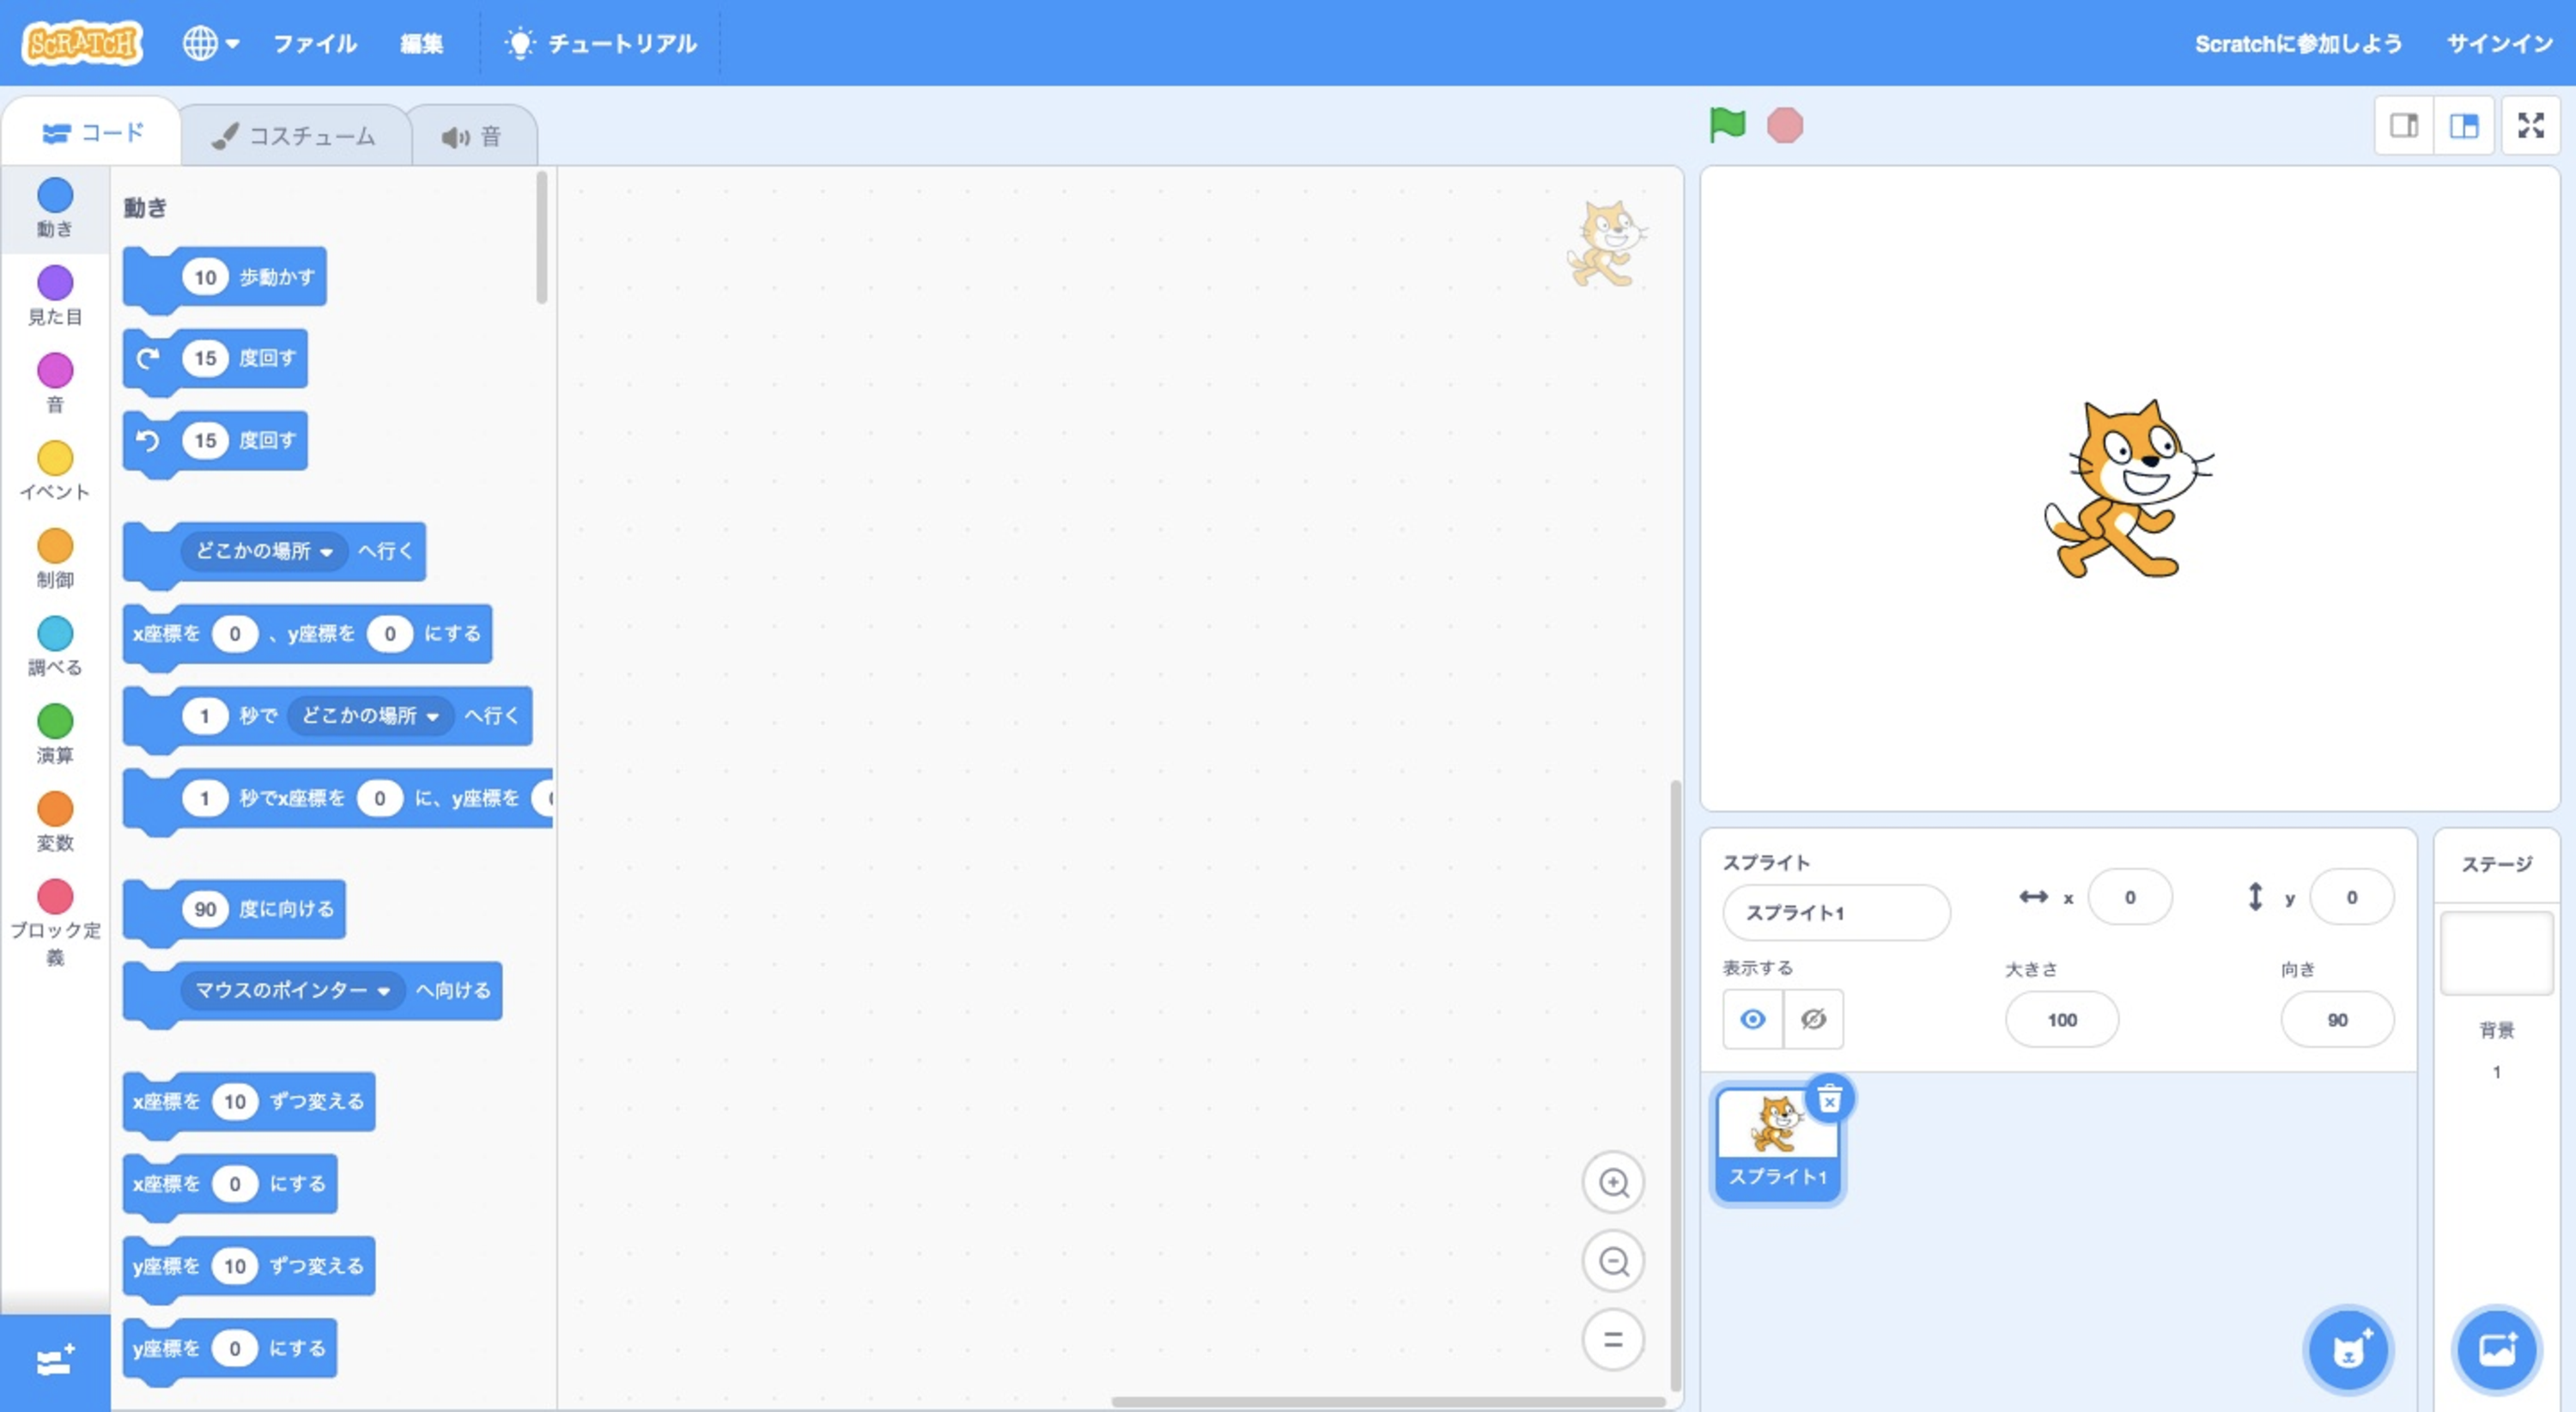
\includegraphics[width=100mm]{images/scratch.pdf}
  \caption{Scrachの実行環境}
  \label{fig:scratch}
\end{figure}

\subsubsection{JavaScript}
JavaScriptとは,Webサイトやシステム開発などで用いられるテキストプログラミング言語である.JavaScriptはとても汎用的なプログラミング言語で,HTMLやCSSと組み合わせて使用することでブラウザ上での動的な処理を実現したり,Node.jsなどのブラウザ側だけでなくサーバー側でも使用される.

本言語では,イベント処理の実現のためにpromiseとthenの仕組みを参考にしている.

\subsubsection{Ruby}
Rubyとは,まつもとゆきひろ氏が作り上げた日本製のテキストプログラミング言語である.主にWeb開発やスマートフォンアプリ開発などに利用されている.Rubyの特徴として,シンプルな記述方法が挙げられる.

本言語では,シンプルな記述によるコードを読んだときに処理の内容のわかりやすさを参考にしている.
\subsubsection{Smalltalk}
Smalltalkとは,手続き型の純粋オブジェクト指向プログラミング言語および実行環境のことを指す.Smalltalkの特徴として,メッセージという仕組みよる文法のシンプルさが挙げられる.メッセージは,メッセージセレクターと0個以上の引数を持っており,それをレシーバに送ることで処理を返す.メッセージには,単項メッセージと二項メッセージ,キーワードメッセージの三種類の形式がある.

プログラム\ref{smalltalk01}にメッセージのプログラム例を示す.1行目は単項メッセージで,レシーバである「10」へ「printString」というメッセージセレクターを送ることで,「10」を文字列に変換した「'10'」の生成を行う.2行目は二項メッセージで,レシーバである「10」へ「+」というメッセージセレクターと引数「5」を送ることで,「10」に「5」を加算し,「15」の生成を行う.3行目はキーワードメッセージで,レシーバである配列「anArray」へ「at:put:」というメッセージセレクターと引数「1」と引数「10」を送ることで,配列「anArray」の1番目の要素を「10」にしている.

本言語では,メッセージによる文法のシンプルさを参考にしている.

\begin{lstlisting}[caption=メッセージのプログラム例, label=smalltalk01]
10 printString.
10 + 5.
anArray at: 1 put: 10.
\end{lstlisting}
\clearpage

\section{言語仕様}
\subsection{概要}
前章において紹介したコンセプトや先行研究\cite{senkou1,senkou2}をもとに,言語仕様を作成した.
簡単な英単語や処理の流れのわかりやすさを重視している.
\subsection{データ型}
本言語におけるデータ型の種類について示す.
\subsubsection{数値型}
数値型は,「5」や「1.5」などの数値で表される.
数値型には二種類あり,整数型と浮動小数点数型の二種類がある.また,数値に対して「-」を先頭につけることで負の数を表すことができる.プログラム\ref{code01}に数値型のプログラム例を示す.

\begin{lstlisting}[caption=数値型のプログラム例, label=code01]
5 -> int;
-5 -> minus;
1.5 -> float;
\end{lstlisting}

\subsubsection{文字列型}
文字列型は,ダブルクォート「"」やシングルクォート「'」で囲まれた文字,数字,記号で表される.プログラム\ref{code02}に文字列型のプログラム例を示す.

\begin{lstlisting}[caption=文字列型のプログラム例, label=code02]
"Hello, World!!" -> str1;
'こんにちは!' -> str2;
\end{lstlisting}

\subsubsection{論理型}
論理型は,真偽値である「true」および「false」で表される.

\subsubsection{範囲型}
範囲型は,「開始値~終端値」で表される.チルダ演算子「~」の左右の開始値と終端値には数値が入り,開始値から終端値までの範囲を生成する.
繰り返し処理であるeachメソッドで使用される.

\begin{lstlisting}[caption=範囲型のプログラム例, label=code03]
{1~10}.each ()=>{};
\end{lstlisting}

\subsubsection{配列型}
配列型は,角括弧「[]」の中身をカンマ「,」で区切ることで表される.プログラム\ref{code04}に配列型のプログラム例を示す.

\begin{lstlisting}[caption=範囲型のプログラム例, label=code04]
[1,2,3,4,5] -> arr;
["a",0,"b"] -> arr;
\end{lstlisting}

\subsection{演算子}
\subsubsection{代入演算子}
代入演算子は,右矢印「->」で表される.右矢印の左側のデータを右側の変数に代入することができる.プログラム\ref{code05}に代入演算子のプログラム例を示す.

\begin{lstlisting}[caption=代入演算子のプログラム例, label=code05]
123 -> num;
"abc" -> str;
[1,2,3] -> arr;
\end{lstlisting}

\subsubsection{パイプライン演算子}
パイプライン演算子は,記号「|>」で表される.記号の左側の値を右側の関数の引数として実行する.関数を連続で実行する場合,左から優先的に実行される.パイプライン演算子を使用することでシンプルに記述することができる.プログラム\ref{code06}にパイプライン演算子のプログラム例を示す.

\begin{lstlisting}[caption=パイプライン演算子のプログラム例, label=code06]
1 |> func;
{a, b} |> func1 |> func2;
\end{lstlisting}

\subsubsection{チルダ演算子}
チルダ演算子は,チルダ「~」で表される.記号の左側が開始値,右側が終端値の範囲型の値を生成する.プログラム\ref{code07}にチルダ演算子のプログラム例を示す.

\begin{lstlisting}[caption=チルダ演算子のプログラム例, label=code07]
1~10;
0 -> start;
start~10;
\end{lstlisting}

\subsubsection{算術演算子}
算術演算子は,数値型の値を用いて算術演算を実行する.表\ref{tab:table01}に算術演算子の一覧を,プログラム\ref{code08}に算術演算子のプログラム例を示す.

\begin{table}[H]
 \caption{算術演算子一覧}
 \label{tab:table01}
 \centering
  \begin{tabular}{cc}
   \hline
   演算子 & 名称 \\
   \hline \hline
   + & 加算演算子 \\
   - & 減算演算子 \\
   \ast & 乗算演算子 \\
   / & 除算演算子 \\
   \% & 余剰演算子 \\
   \hline
  \end{tabular}
\end{table}

\begin{lstlisting}[caption=算術演算子のプログラム例, label=code08]
10 + 10;
10 - 10;
10 * 10; 
10 / 10;
10 % 10;
\end{lstlisting}

\subsubsection{比較演算子}
比較演算子は,二つの値の比較を行い,結果として真偽値を返す.表\ref{tab:table02}に比較演算子の一覧を,プログラム\ref{code09}に比較演算子のプログラム例を示す.

\begin{table}[H]
 \caption{比較演算子一覧}
 \label{tab:table02}
 \centering
  \begin{tabular}{cc}
   \hline
   演算子 & 名称 \\
   \hline \hline
   = & 等価演算子 \\
   <= & 以下演算子 \\
   >= & 以上演算子 \\
   < & 小なり演算子 \\
   > & 大なり演算子 \\
   \hline
  \end{tabular}
\end{table}

\begin{lstlisting}[caption=比較演算子のプログラム例, label=code09]
10 = 10;
10 <= 100;
100 >= 10; 
10 < 100;
100 > 10;
\end{lstlisting}

\subsubsection{論理演算子}
論理演算子は,真偽値に対して論理演算を行う.表\ref{tab:table03}に論理演算子の一覧を,プログラム\ref{code10}に論理演算子のプログラム例を示す.

\begin{table}[H]
 \caption{論理演算子一覧}
 \label{tab:table03}
 \centering
  \begin{tabular}{cc}
   \hline
   演算子 & 名称 \\
   \hline \hline
   and & AND演算子 \\
   or & OR演算子 \\
   \hline
  \end{tabular}
\end{table}

\begin{lstlisting}[caption=論理演算子のプログラム例, label=code10]
true and true;
true or false;
\end{lstlisting}

\subsection{変数}
変数を宣言する場合,必ず初期化が必要となる.代入演算子を用いて,データを変数に代入することで,変数を宣言することができる.プログラム\ref{code11}に変数のプログラム例を示す.

\begin{lstlisting}[caption=変数のプログラム例, label=code11]
100 -> num;
() => {} -> func;
{10, 20} |> func -> ans; 
\end{lstlisting}

\subsection{関数}
関数とは,一連の処理をまとめたものを表す.関数の宣言には,ラムダ式を用いる.括弧「()」内に引数を,中括弧「\{\}」内に処理を記述する.また,returnで戻り値を指定する.関数は変数に代入することもできる.プログラム\ref{code12}に関数のプログラム例を示す.

\begin{lstlisting}[caption=関数のプログラム例, label=code12]
(a,b) => { return a + b } -> add;
{10, 20} |> add;
\end{lstlisting}

\subsection{クラス}
クラスとは,オブジェクトの設計図に相当するものである.SpliteクラスやStageクラスなどが存在する.クラスは大文字から始まる.

\subsection{メソッド}
メソッドとは,あるオブジェクトに対する手続きのことを指す.「オブジェクト名.メソッド パラメータ」で表される.メソッドを使用することで,スプライトの動作,見た目の変更などの処理を行う.プログラム\ref{code13}にクラスとメソッドのプログラム例を示す.例では,Spliteクラスにあるnewメソッドにより,cat内に「ねこ」という名前のスプライトを生成している.また,walkメソッドを使用し,生成したスプライトを10歩進ませる処理を行なっている.

\begin{lstlisting}[caption=クラスとメソッドのプログラム例, label=code13]
Splite.new name:"ねこ"-> cat;
cat.walk 10; 
\end{lstlisting}

\subsection{構文規則}

\clearpage

\section{Scratchとの比較}
Scratchのブロックは指示の種類に分類されており,「動き」,「見た目」,「音」,「イベント」,「制御」,「調べる」,「演算」等の種類がある.現時点では,全ての機能を本言語内で取り扱うことは想定しておらず,必要最低限の機能の実装を想定している.種類ごとにScratchのブロックと本言語の記述の比較したものを示す.

\subsection{動き}
Scratchにおける「動き」に関連するブロックと本言語における類似した処理との比較を以下に示す.
\subsubsection{walkメソッド}
図\ref{fig:walk}で示されたScratchにおける「〜歩動かす」ブロックは,スプライトの向いている方向への移動処理を行う.本言語では,walkメソッドにより同様の処理を行う.

walkメソッドは,「スプライト名.walk」で向いている方向へ,指定した数値分の移動を行う.プログラム\ref{code14}にwalkメソッドのプログラム例を示す.

\begin{figure}[H]
  \centering
  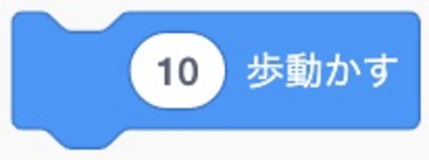
\includegraphics[height=15mm]{images/walk.pdf}
  \caption{「〜歩動かす」ブロック}
  \label{fig:walk}
\end{figure}

\begin{lstlisting}[caption=walkメソッドのプログラム例, label=code14]
Splite.new name:"ねこ" -> cat;
cat.walk 50; 
\end{lstlisting}

\subsubsection{moveメソッド}

図\ref{fig:move}で示されたScratchにおける「座標を〜にする」ブロックは,スプライトの元座標から指定した座標への移動処理を行う.また,移動にかける時間も指定することができる.本言語では,moveメソッドで同様の処理を行う.

moveメソッドは,「スプライト名.move」でx座標の値,y座標の値,時間を指定し,指定された座標への移動処理を行う.プログラム\ref{code15}にmoveメソッドのプログラム例を示す.

\begin{figure}[H]
  \centering
  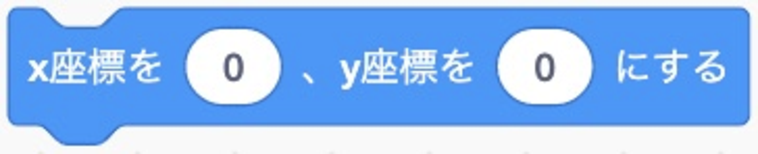
\includegraphics[height=15mm]{images/move_x_y.pdf} \\
  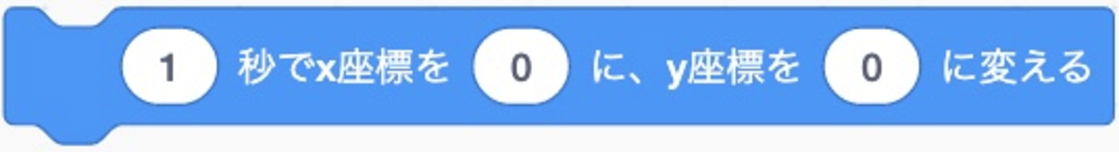
\includegraphics[height=15mm]{images/move_x_y_time.pdf} \\
  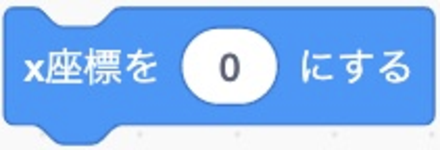
\includegraphics[height=15mm]{images/move_x.pdf} \\
  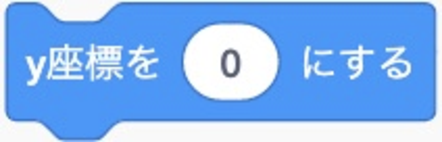
\includegraphics[height=15mm]{images/move_y.pdf} 
  \caption{「座標を〜にする」ブロック}
  \label{fig:move}
\end{figure}

\begin{lstlisting}[caption=moveメソッドのプログラム例, label=code15]
Splite.new name:"ねこ" -> cat;
cat.move x:10, y:10, time:2; 
\end{lstlisting}

\subsubsection{move\_stepメソッド}
図\ref{fig:step}で示されたScratchにおける「座標を〜ずつ変える」ブロックは,スプライトの元座標から指定した値分の座標移動を行う.本言語では,move\_stepメソッドで同様の処理を行う.

move\_stepメソッドは,「スプライト名.move\_step」でx座標の変化量,またはy座標の変化量を指定し,指定された値分の移動処理を行う.正負どちらの値も指定することができる.プログラム\ref{code16}にmove\_stepメソッドのプログラム例を示す.

\begin{figure}[H]
  \centering
  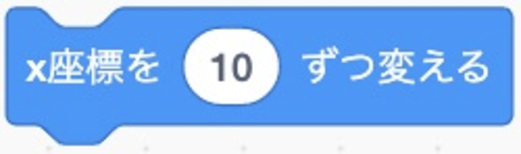
\includegraphics[height=15mm]{images/step_x.pdf} 
  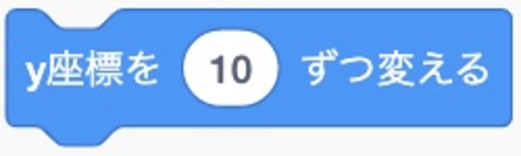
\includegraphics[height=15mm]{images/step_y.pdf} 
  \caption{「座標を〜ずつ変える」ブロック}
  \label{fig:step}
\end{figure}

\begin{lstlisting}[caption=move\_stepメソッドのプログラム例, label=code16]
Splite.new name:"ねこ" -> cat;
cat.move_step x:10; 
cat.move_step y:-10; 
\end{lstlisting}

\subsubsection{turnメソッド}
図\ref{fig:turn}で示されたScratchにおける「〜度回す」,「〜度に向ける」ブロックは,スプライトの向きの変更を行う.本言語では,turnメソッドで同様の処理を行う.

turnメソッドは,「スプライト名.turn」で角度を変更することができる.向きは0度から360度まであり,0度と360度が上向き,90度が右向き,180度が下向き,240度が左向きを表す.正負の値どちらも指定することができる.プログラム\ref{code17}にturnメソッドのプログラム例を示す.

\begin{figure}[H]
  \centering
  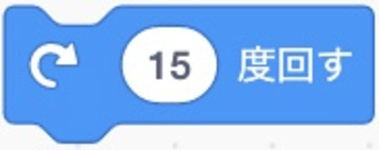
\includegraphics[height=15mm]{images/turn_right.pdf} 
  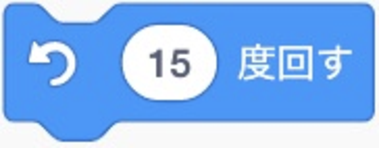
\includegraphics[height=15mm]{images/turn_left.pdf} 
  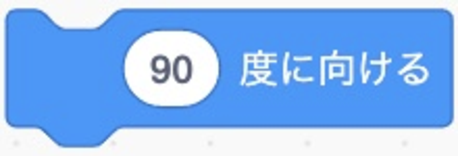
\includegraphics[height=15mm]{images/turn.pdf}
  \caption{「〜度回す」,「〜度に向ける」ブロック}
  \label{fig:turn}
\end{figure}

\begin{lstlisting}[caption=turnメソッドのプログラム例, label=code17]
Splite.new name:"ねこ" -> cat;
cat.turn 90;
cat.turn -180; 
\end{lstlisting}

\subsubsection{returnメソッド}
図\ref{fig:return}で示されたScratchにおける「もし端に着いたら,跳ね返る」ブロックは,スプライトがステージの外枠に触れた時,スプライトの向きを反転させる.本言語では,条件分岐とtouchメソッド,returnメソッドで処理を再現する.

touchメソッドとは,二つのオブジェクト同士が接触しているかどうかを真偽値で返すKnowクラスのメソッドである.また,returnメソッドとは,接触しているステージの端に接触しているとき,スプライトの向きを逆にするメソッドである.プログラム\ref{code18}にreturnメソッドのプログラム例を示す.プログラム\ref{code18}では,ステージの外枠とスプライトが接触しているかどうかを判定している.そして,if文でtrueが与えられた場合は,returnメソッドで跳ね返り処理を行う.

\begin{figure}[H]
  \centering
  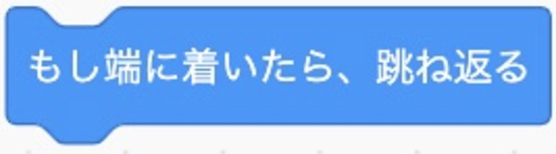
\includegraphics[height=15mm]{images/return.pdf}
  \caption{「もし端に着いたら,跳ね返る」ブロック}
  \label{fig:return}
\end{figure}

\begin{lstlisting}[caption=returnメソッドのプログラム例, label=code18]
Stage.new name:"いえ" -> stage;
Splite.new name:"ねこ" -> cat;
{ cat.touch stage.around }.if {
  cat.return;
};
\end{lstlisting}

\subsubsection{xメソッドとyメソッド}
図\ref{fig:xy}で示されたScratchにおける「座標」ブロックは,あるスプライトが所持している座標情報を呼び出すことができる.本言語では,xメソッドとyメソッドで同様の処理を行う.

xメソッドとyメソッドは,「スプライト名.x」と「スプライト名.y」でそれぞれスプライトのx座標の値とy座標の値を呼び出す.プログラム\ref{code19}にxメソッドとyメソッドのプログラム例を示す.

\begin{figure}[H]
  \centering
  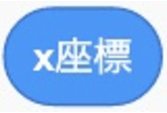
\includegraphics[height=15mm]{images/x.pdf} 
  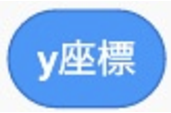
\includegraphics[height=15mm]{images/y.pdf} 
  \caption{「座標」ブロック}
  \label{fig:xy}
\end{figure}

\begin{lstlisting}[caption=xメソッドとyメソッドのプログラム例, label=code19]
Splite.new name:"ねこ", x:10, y:-10 -> cat;
cat.x -> num_x;
cat.x -> num_y;
\end{lstlisting}
\subsection{見た目}
Scratchにおける「見た目」に関連するブロックと本言語における類似処理との比較を以下に示す.

\subsubsection{sayメソッド}
図\ref{fig:say}で示されたScratchにおける「〜と言う」「〜と考える」ブロックは,スプライトの頭上に吹き出しと台詞を表示させる.本言語では,sayメソッドで「〜と言う」ブロックと同様の処理を行う.「〜と言う」ブロックと「〜と考える」ブロックの違いは吹き出しの形状のみなので,同一のものとして考えている.

sayメソッドは,「スプライト名.say」で文字列のデータを与えることで,スプライトの頭上に吹き出しを表示する.プログラム\ref{code20}にsayメソッドのプログラム例を示す.sayメソッドは実行された場合,常に吹き出しが表示され続ける.そのため,吹き出しを消す場合は,「スプライト名.say ""」のように,空の文字列を与えることで上書きする必要がある.プログラム\ref{code20}では,「こんにちは!」を表示してから3秒後に吹き出しを消すという処理を行なっている.

\begin{figure}[H]
  \centering
  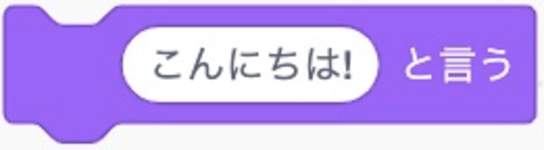
\includegraphics[height=15mm]{images/say.pdf} \\
  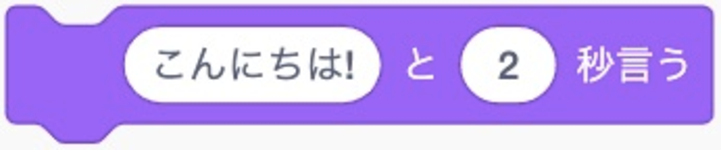
\includegraphics[height=15mm]{images/say_time.pdf} \\
  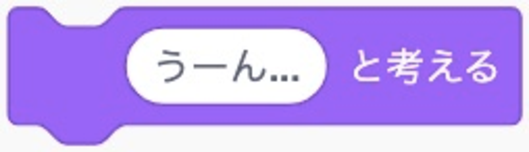
\includegraphics[height=15mm]{images/think.pdf} \\
  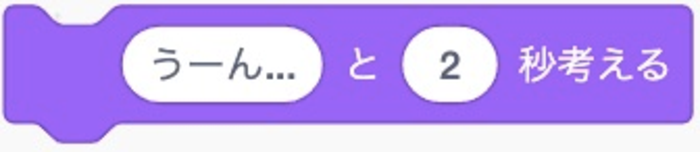
\includegraphics[height=15mm]{images/think_time.pdf} 
  \caption{「〜と言う」「〜と考える」ブロック}
  \label{fig:say}
\end{figure}

\begin{lstlisting}[caption=sayメソッドのプログラム例, label=code20]
Splite.new name:"ねこ" -> cat;
cat.say "こんにちは!";
{ 3.second }.wait;
cat.say "";
\end{lstlisting}

\subsubsection{costumeメソッドとnext\_costumeメソッド}
図\ref{fig:costume}で示されたScratchにおける「コスチュームを〜にする」ブロックは,スプライトの所持している「コスチューム」という差分イラストへの変更処理を行う.本言語では,costumeメソッドとnext\_costumeメソッドで同様の処理を行う.

本言語では,Spliteクラスに事前にスプライトのイラストやコスチュームが用意されている.コスチュームにはそれぞれ番号と名前が割り当てられている.costumeメソッドでは,「スプライト名.costume」で番号か名前を指定することで,コスチュームの変更を行う.

また,next\_costumeメソッドでは,「スプライト名.next\_costume」で次の番号のコスチュームへの変更を行う.プログラム\ref{code21}にcostumeメソッドとnext\_costumeメソッドのプログラム例を示す.

\begin{figure}[H]
  \centering
  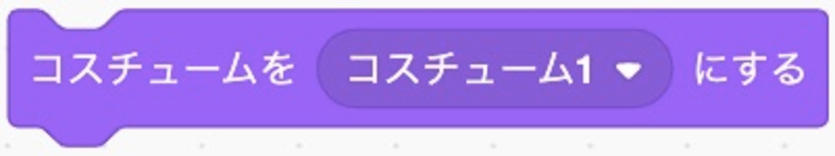
\includegraphics[height=15mm]{images/wear.pdf} \\
  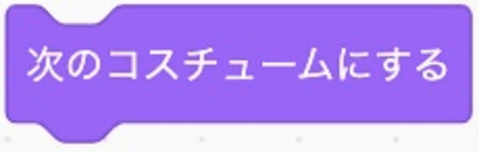
\includegraphics[height=15mm]{images/next_wear.pdf} 
  \caption{「コスチュームを〜にする」ブロック}
  \label{fig:costume}
\end{figure}

\begin{lstlisting}[caption=costumeメソッドとnext\_costumeメソッドのプログラム例, label=code21]
Splite.new name:"ねこ" -> cat;
cat.costume "コスチューム1";
cat.next_costume;
\end{lstlisting}

\subsubsection{backgroundメソッドとnext\_backgroundメソッド}
図\ref{fig:background}で示されたScratchにおける「背景を〜にする」ブロックは,ステージの所持している「背景」という差分イラストへの変更処理を行う.本言語では,backgroundメソッドとnext\_backgroundメソッドで同様の処理を行う.

本言語では,Stageクラスに事前にステージのイラストや背景が用意されている.背景にはそれぞれ番号と名前が割り当てられている.backgroundメソッドでは,「ステージ名.background」で番号か名前を指定することで,背景の変更を行う.

また,next\_backgroundメソッドでは,「スプライト名.next\_background」で次の番号のコスチュームへの変更を行う.プログラム\ref{code22}にcostumeメソッドとnext\_backgroundメソッドのプログラム例を示す.

\begin{figure}[H]
  \centering
  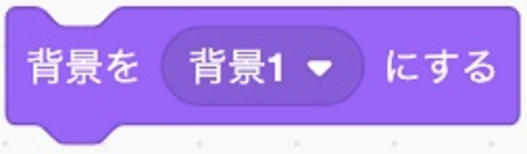
\includegraphics[height=15mm]{images/set.pdf} \\
  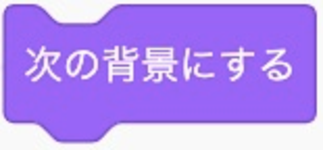
\includegraphics[height=15mm]{images/next_set.pdf} 
  \caption{「背景を〜にする」ブロック}
  \label{fig:background}
\end{figure}

\begin{lstlisting}[caption=backgroundメソッドとnext\_backgroundメソッドのプログラム例, label=code22]
Stage.new name:"ステージ" -> stage;
stage.background "ゆき";
stage.next_background;
\end{lstlisting}

\subsubsection{sizeメソッド}
図\ref{fig:size}で示されたScratchにおける「大きさを〜\%にする」ブロックは,スプライトの大きさを変更する処理を行う.本言語では,sizeメソッドで同様の処理を行う.

sizeメソッドは,「スプライト名.size」で変更する大きさを指定する.標準サイズは100\%である.プログラム\ref{code23}にsizeメソッドのプログラム例を示す.

\begin{figure}[H]
  \centering
  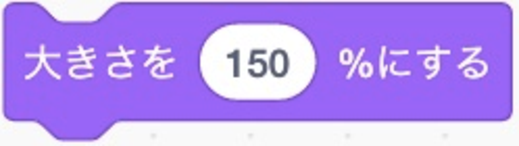
\includegraphics[height=15mm]{images/size.pdf}
  \caption{「大きさを〜\%にする」ブロック}
  \label{fig:size}
\end{figure}

\begin{lstlisting}[caption=sizeメソッドのプログラム例, label=code23]
Splite.new name:"ねこ" -> cat;
cat.size 150;
\end{lstlisting}

\subsubsection{size\_stepメソッド}
図\ref{fig:size_step}で示されたScratchにおける「大きさを〜\%にする」ブロックは,スプライトの大きさを指定した値分の変更を行う.本言語では,size\_stepメソッドで同様の処理を行う.

size\_stepメソッドは,「スプライト名.size\_step」で変化量を指定する.正負の値どちらも指定することができる.プログラム\ref{code24}にsize\_stepメソッドのプログラム例を示す.

\begin{figure}[H]
  \centering
  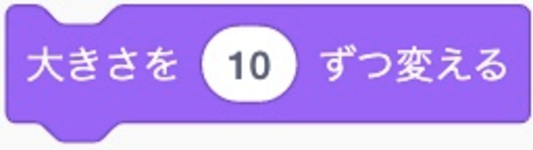
\includegraphics[height=15mm]{images/size_step.pdf}
  \caption{「大きさを〜ずつ変える」ブロック}
  \label{fig:size_step}
\end{figure}

\begin{lstlisting}[caption=size\_stepメソッドのプログラム例, label=code24]
Splite.new name:"ねこ" -> cat;
cat.size_step 10;
\end{lstlisting}

\subsubsection{showメソッド}
図\ref{fig:show}で示されたScratchにおける「表示」ブロックはスプライトを表示し,「非表示」ブロックはスプライトを非表示にする.本言語では,showメソッドで同様の処理を行う.

showメソッドは,「スプライト名.show」に真偽値を与えることで,表示と非表示の変更を行う.trueが与えられたとき,スプライトを表示し,falseが与えられたとき,スプライトを非表示にする.プログラム\ref{code25}にshowメソッドのプログラム例を示す.

\begin{figure}[H]
  \centering
  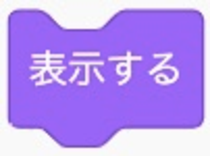
\includegraphics[height=15mm]{images/show.pdf} 
  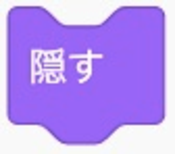
\includegraphics[height=15mm]{images/hide.pdf}
  \caption{「表示」「非表示」ブロック}
  \label{fig:show}
\end{figure}

\begin{lstlisting}[caption=showメソッドのプログラム例, label=code25]
Splite.new name:"ねこ" -> cat;
cat.show true;
cat.show false;
\end{lstlisting}

\subsection{イベント}
Scratchにおける「イベント」に関連するブロックと本言語における類似処理との比較を以下に示す.
図\ref{fig:then}で示されたScratchにおける「〜されたとき」ブロックは,イベント処理を表す.本言語では,KeyEventクラスやClickEventクラスやMessageEventクラスとifメソッドを使用することで処理を再現している.JavaScriptにおけるPromiseを利用した非同期処理の仕組みを参考にしている.

プログラム\ref{code26}にイベント処理のプログラム例を示す.「ClickEvent.new」でクラスのインスタンス「ev」を作成している.ClickEventクラスのインスタンスは,クリックしたオブジェクトのキーワードを受け取る.プログラム\ref{code26}では,旗が押されたときに発行される「flag」を受け取っており,ifメソッドでflagを受け取ったときの処理を記述している.

KeyEventクラスのインスタンスは,キーが押されたときにキーの名前を,ClickEventクラスのインスタンスは,スプライトがクリックされたときにスプライトの名前をキーワードとして受け取る.

また,図\ref{fig:send}で示されたScratchにおける「〜を送る」「〜を送って待つ」ブロックは,Scratchプロジェクト全体にメッセージを送る.本言語では,メッセージを送る場合は,MessageEventクラスのインスタンスにパイプライン演算子でメッセージを送る.

\begin{figure}[H]
  \centering
  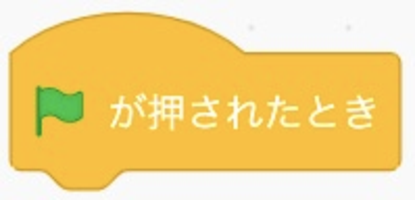
\includegraphics[height=15mm]{images/flag.pdf} 
  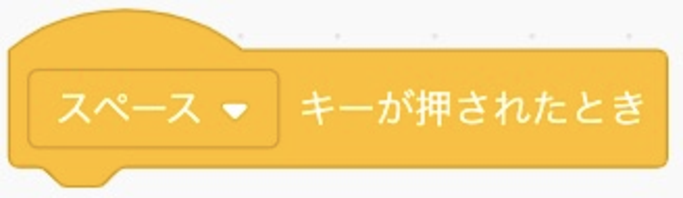
\includegraphics[height=15mm]{images/keypress.pdf} \\
  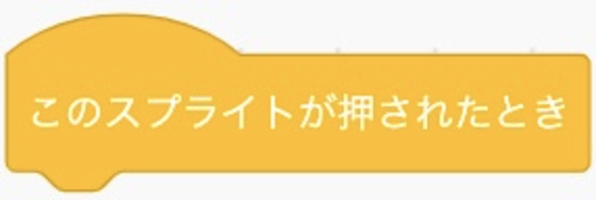
\includegraphics[height=15mm]{images/click.pdf} 
  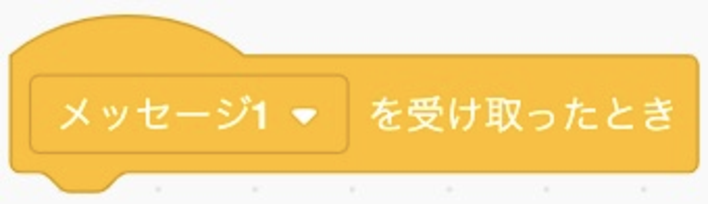
\includegraphics[height=15mm]{images/message.pdf}
  \caption{「〜されたとき」ブロック}
  \label{fig:then}
\end{figure}

\begin{figure}[H]
  \centering
  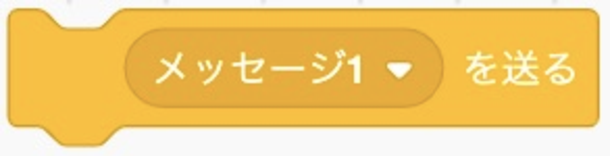
\includegraphics[height=15mm]{images/send.pdf} 
  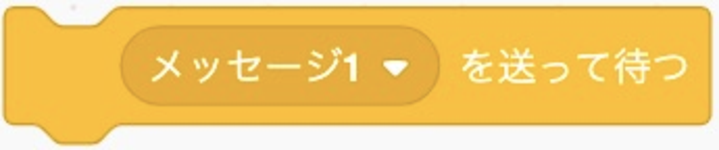
\includegraphics[height=15mm]{images/send2.pdf} 
  \caption{「〜送る」「〜を送って待つ」ブロック}
  \label{fig:send}
\end{figure}

\begin{lstlisting}[caption=イベント処理のプログラム例, label=code26]
Splite.new name:"ねこ" -> cat;
ClickEvent.new -> click;
MessageEvent.new -> mes;
{ click = "flag" }.if {
  cat.say "こんにちは!";
  終了 |> mes;
};
\end{lstlisting}

\subsection{制御}
Scratchにおける「制御」に関連するブロックと本言語における類似処理との比較を以下に示す.
\subsubsection{waitメソッド}
図\ref{fig:wait}で示されたScratchにおける「〜秒待つ」ブロックは,スクリプトの一時停止を行う.「〜を止める」ブロックは指定したスクリプトの停止を行う.本言語では,waitメソッドで「〜秒待つ」ブロックの処理を再現している.

waitメソッドは,「スプライト名.wait」で指定した時間分のスプライトの一時停止を行う.プログラム\ref{code27}にwaitメソッドのプログラム例を示す.

\begin{figure}[H]
  \centering
  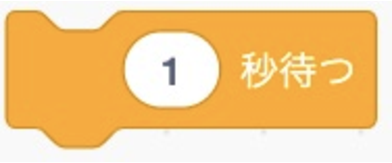
\includegraphics[height=15mm]{images/wait.pdf} \\
  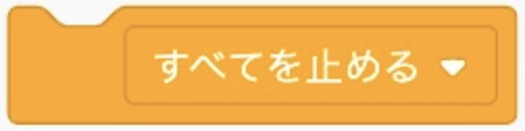
\includegraphics[height=15mm]{images/stop.pdf} 
  \caption{「〜秒待つ」「〜を止める」ブロック}
  \label{fig:wait}
\end{figure}

\begin{lstlisting}[caption=waitメソッドのプログラム例, label=code27]
Splite.new name:"ねこ" -> cat;
cat.wait 60;
\end{lstlisting}

\subsubsection{eachメソッド}
図\ref{fig:each}で示されたScratchにおける「〜回繰り返す」ブロックは,指定した回数分の繰り返し処理を行う.本言語では,eachメソッドで同様の処理を行う.

eachメソッドは,「範囲型.each 処理」のように,範囲型で示された回数分,指定された処理を行う.プログラム\ref{code28}にeachメソッドのプログラム例を示す.範囲型の開始値から終端値までが処理の引数に与えられる.

\begin{figure}[H]
  \centering
  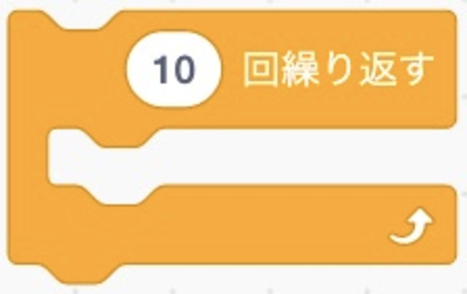
\includegraphics[height=30mm]{images/each.pdf} 
  \caption{「〜回繰り返す」ブロック}
  \label{fig:each}
\end{figure}

\begin{lstlisting}[caption=eachメソッドのプログラム例, label=code28]
0 -> sum;
{ 1~10 }.each (i) => {
  sum + i -> sum;
};
\end{lstlisting}
\subsubsection{whileメソッド}
図\ref{fig:while}で示されたScratchにおける「〜まで繰り返す」ブロックは,指定した条件が真になるまで繰り返し処理を行う.本言語では,whileメソッドで類似した処理を行う.

whileメソッドは,「条件式.while 処理」のように,条件式の結果がtrueである間,指定された処理を行う.プログラム\ref{code29}にwhileメソッドのプログラム例を示す.

\begin{figure}[H]
  \centering
  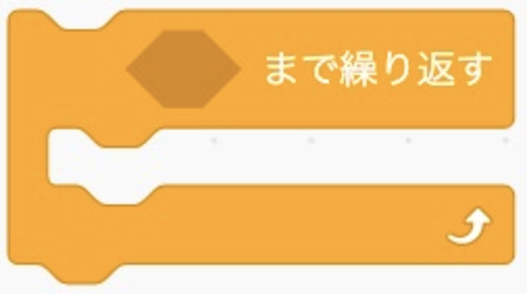
\includegraphics[height=30mm]{images/while.pdf} 
  \caption{「〜まで繰り返す」ブロック}
  \label{fig:while}
\end{figure}

\begin{lstlisting}[caption=whileメソッドのプログラム例, label=code29]
10 -> num;
{ num > 0 }.while {
  num - 1 -> num;
};
\end{lstlisting}

また,図\ref{fig:while}で示されたScratchにおける「ずっと繰り返す」ブロックは,無限ループを行う.whileメソッドは,「true.while」とすることで,永続的な繰り返し処理を行う.「break」で無限ループから抜け出すことができる.プログラム\ref{code30}に無限ループのプログラム例を示す.

\begin{figure}[H]
  \centering
  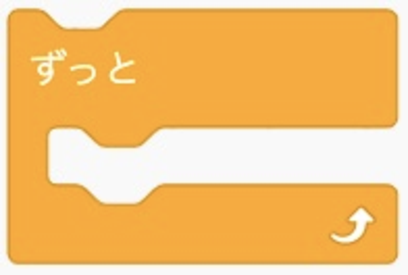
\includegraphics[height=25mm]{images/truewhile.pdf} 
  \caption{「ずっと繰り返す」ブロック}
  \label{fig:while}
\end{figure}

\begin{lstlisting}[caption=無限ループのプログラム例, label=code30]
0 -> sum;
true.while {
  sum + 1 -> sum;
  { sum > 10 }.if {
    break;
  };
};
\end{lstlisting}
\subsubsection{ifメソッド}
図\ref{fig:if}で示されたScratchにおける「もし〜ならば」ブロックは,指定した条件が真である場合のみ処理を行う.本言語では,ifメソッドで類似した処理を行う.

ifメソッドは,「条件式.if 処理」のように,条件式の結果がtrueである場合,処理を行う.プログラム\ref{code31}にifメソッドのプログラム例を示す.

\begin{figure}[H]
  \centering
  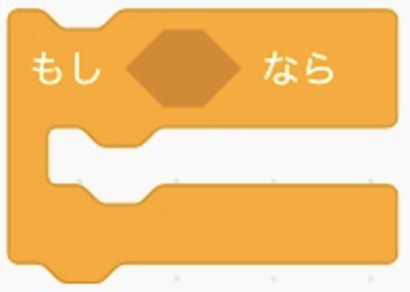
\includegraphics[height=30mm]{images/if.pdf}
  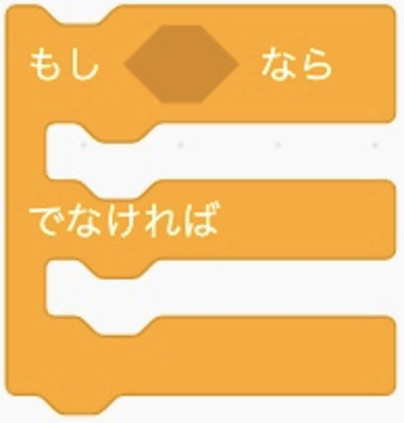
\includegraphics[height=45mm]{images/if2.pdf} 
  \caption{「もし〜ならば」ブロック}
  \label{fig:if}
\end{figure}

\begin{lstlisting}[caption=ifメソッドのプログラム例, label=code31]
3 -> num;
{num = 3}.if { 
  0 -> num;
};
\end{lstlisting}

\subsection{調べる}
Scratchにおける「調べる」に関連するブロックと本言語における類似処理との比較を以下に示す.
\subsubsection{touchメソッド}
図\ref{fig:touch}で示されたScratchにおける「〜に触れた」ブロックは,スプライトがある要素に対して接触したかどうかの判定処理を行う.本言語では,touchメソッドで同様の処理を行う.

touchメソッドでは,接触したかの判定をしたい要素をtouchメソッドに与えることで,その結果を真偽値で返す.プログラム\ref{code32}にtouchメソッドのプログラム例を示す.
\begin{figure}[H]
  \centering
  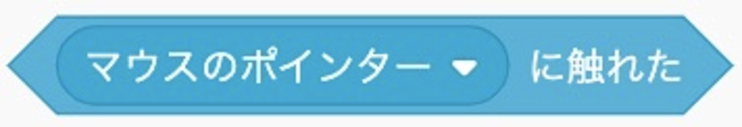
\includegraphics[height=15mm]{images/touch.pdf}
  \caption{「〜に触れた」ブロック}
  \label{fig:touch}
\end{figure}

\begin{lstlisting}[caption=touchメソッドのプログラム例, label=code32]
Splite.new name:"ねこ" -> cat;
Splite.new name:"いぬ" -> dog;
cat.touch dog;
\end{lstlisting}

\subsubsection{length\_betweenメソッド}
図\ref{fig:length}で示されたScratchにおける「〜までの距離」ブロックは,スプライトとある要素との距離を返す.本言語では,length\_betweenメソッドで同様の処理を行う.

length\_betweenメソッドでは,二つのスプライト間の距離を数値で返す.プログラム\ref{code33}にlength\_betweenメソッドのプログラム例を示す.

\begin{figure}[H]
  \centering
  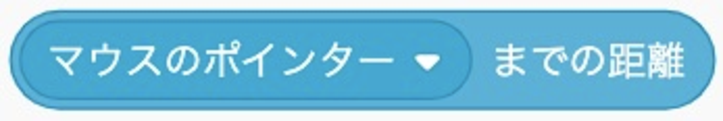
\includegraphics[height=15mm]{images/mouse.pdf}
  \caption{「〜までの距離」ブロック}
  \label{fig:length}
\end{figure}

\begin{lstlisting}[caption=length\_betweenメソッドのプログラム例, label=code33]
Splite.new name:"ねこ" -> cat;
Splite.new name:"いぬ" -> dog;
cat.length_between dog;
\end{lstlisting}

\subsubsection{mouse\_xメソッドとmouse\_yメソッド}
図\ref{fig:length}で示されたScratchにおける「マウスの座標」ブロックは,マウスのカーソルの座標の値を持っている.本言語では,mouse\_xメソッドとmouse\_yメソッドで同様の処理を行う.

mouse\_xメソッドは,マウスのx座標の値を呼び出す.mouse\_yメソッドは,マウスのy座標の値を呼び出す.プログラム\ref{code34}にmouse\_xメソッドとmouse\_yメソッドのプログラム例を示す.

\begin{figure}[H]
  \centering
  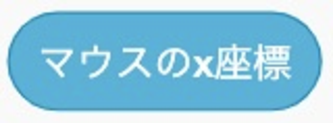
\includegraphics[height=15mm]{images/mouse_x.pdf} 
  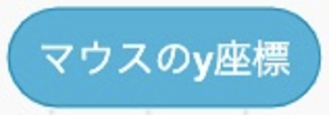
\includegraphics[height=15mm]{images/mouse_y.pdf} 
  \caption{「マウスの座標」ブロック}
  \label{fig:length}
\end{figure}

\begin{lstlisting}[caption=mouse\_xメソッドとmouse\_yメソッドのプログラム例, label=code34]
kn.mouse_x -> num_x;
kn.mouse_y -> num_y;
\end{lstlisting}

\subsection{演算}
Scratchにおける「調べる」に関連するブロックと本言語における類似処理との比較を以下に示す.
\subsubsection{算術演算}
図\ref{fig:math}で示されたScratchにおける「算術演算」ブロックは,算術演算を行う.本言語では,表\ref{tab:table01}に示された算術演算子を用いる.

\begin{figure}[H]
  \centering
  
\includegraphics[height=15mm]{images/add.pdf}
  
\includegraphics[height=15mm]{images/sub.pdf} \\
  
\includegraphics[height=15mm]{images/mul.pdf}
  
\includegraphics[height=15mm]{images/div.pdf} \\
  
\includegraphics[height=15mm]{images/rem.pdf}
  \caption{「算術演算」ブロック}
  \label{fig:math}
\end{figure}

\subsubsection{比較演算}
図\ref{fig:com}で示されたScratchにおける「比較演算」ブロックは,比較演算を行う.本言語では,表\ref{tab:table02}に示された比較演算子を用いる.

\begin{figure}[H]
  \centering
  
\includegraphics[height=15mm]{images/over.pdf}
  
\includegraphics[height=15mm]{images/less.pdf}
  \includegraphics[height=15mm]{images/equ.pdf}
  \caption{「比較演算」ブロック}
  \label{fig:com}
\end{figure}

\subsubsection{論理演算}
図\ref{fig:log}で示されたScratchにおける「論理演算」ブロックは,論理演算を行う.本言語では,表\ref{tab:table03}に示された論理演算子を用いる.

\begin{figure}[H]
  \centering
  \includegraphics[height=15mm]{images/and.pdf}
  \includegraphics[height=15mm]{images/or.pdf}
  \caption{「比較演算」ブロック}
  \label{fig:log}
\end{figure}

\subsubsection{乱数}
図\ref{fig:log}で示されたScratchにおける「〜から〜までの乱数」ブロックは,指定された範囲内の乱数を生成する.本言語では,Randomクラスによって同様の処理を行う.

「Random.new from:開始値, to:終端値」で,開始値から終端値までの乱数を生成する.プログラム\ref{code35}に乱数のプログラム例を示す.

\begin{figure}[H]
  \centering
  \includegraphics[height=15mm]{images/random.pdf}
  \caption{「〜から〜までの乱数」ブロック}
  \label{fig:log}
\end{figure}

\begin{lstlisting}[caption=乱数のプログラム例, label=code35]
Random.new from:1, to:10 -> rand;
rand -> num;
\end{lstlisting}
\clearpage

\section{結言}
%背景
近年の急速な情報化に伴い,2020年度から小学校ではプログラミング教育の必修化が行われた.これにより小学生でも扱いやすいビジュアルプログラミング言語が注目されている.
代表的なビジュアルプログラミング言語に「Scratch」がある.「Scratch」は指示の書かれたブロックを並べることで視覚的にわかりやすく,直感的な操作でプログラミングができる.また,文字のタイピング量が少ない点や英単語の知識を必要としない点などから,初学者のプログラミング学習に適している.

%問題点
本格的なプログラムを作成していくうえで,テキストプログラミング言語の学習が必要になる.しかし,Scratchに慣れていると,テキストプログラミング言語の学習を始めようとしたときに仕様の違いが挫折の要因になり得ると考えた.例えば,スプライトの有無やソースコードの記述方法などが挙げられる.

%先行研究
当研究室ではこれまで,上記の問題点を考慮したテキストプログラミング言語に関する先行研究が行われてきた.内堀は,ビジュアルプログラミングとテキストプログラミングについての調査を行い,初学者向けのテキストプログラミング言語の基礎を示した\cite{senkou1}.また,菅原は,開発するプログラミング言語の言語仕様を定め,インタープリタの開発を行った\cite{senkou2}.

しかし,先行研究の問題点として,開発するプログラミング言語の言語仕様はまとまりきっておらず,インタープリタのパーサーが正しく動作しないなどがある.

%目的
そこで本研究では,Scratchを学んだ学習者が,次の段階として抵抗感を減らすことを目的としたテキストプログラミング言語「Chiba-lang」のコンセプトを定め,サンプルプログラムと言語仕様書の作成を行った.

%今後
今後は,本研究でまとめられた言語仕様より,インタープリタや実行環境の開発を進めていく.
\clearpage

\section{謝辞}
本論文の作成にあたり、多くの方々にご指導ご鞭撻を賜りました。
須田浩准教授や須田研究室の仲間には,多大なる御指導及び御助言を頂きました.深く感謝申し上げます.
\clearpage

\begin{thebibliography}{99}
\bibitem{senkou1} 内掘美幸: ``Scratchからの移行を考慮したプログラミング言語と環境の開発'', 2019年度卒業研究
\bibitem{senkou2} 菅原直輝: ``Scratchからの移行を考慮したプログラミング言語の開発'', 2020年度卒業研究
\bibitem{pdf1} 文部科学省,``小学校プログラミング教育の手引(第三版)'', (2020),\url{https://www.mext.go.jp/content/20200218-mxt_jogai02-100003171_002.pdf}
\end{thebibliography}

\end{document}
